% Chapter 1

\chapter{Theoretical framework} % Chapter title

\label{ch:thfw} % For referencing the chapter elsewhere, use \autoref{ch:name}

%----------------------------------------------------------------------------------------

\section{Motivation}

One of the longstanding questions in hadronic physics is the one concerning the inner structure of the nucleon and in particular its spin structure. Momentum distributions of polarized and unpolarized partons (quarks and gluons) can be described with the polarized and unpolarized Parton Distribution Functions (PDFs). At COMPASS, polarized (resp. upolarized) measurements of Deep Inelastic Scattering (DIS) of longitudinally polarized (resp. unpolarized) muons on longitudinally polarized (resp. unpolarized) nucleons are performed in order to determine the spin structure function of the nucleon as well as to determine which fraction of the nucleon spin is carried by the spin of each parton. To reach this goal SIDIS data with detection of a hadron (pion, kaon or proton), tagging the flavour of the struck quark are taken. This hadronization process is described to the quark Fragmentation Functions (FFs) into hadrons which are themselves useful in the determination of the spin structure functions through SIDIS. These FFs are well known for the first generation of quarks but still not well determined for higher mass quark with a discrepancy up to a factor 3 between parametrizations for the strange quark. They thus constitute the largest uncertainty for the determination of the strange quark polarization in Semi-Inclusive DIS (SIDIS), though in the COMPASS kinematic range, the strange quark PDF is also affected by large uncertainties.

To help improve the situation, the extraction of hadron multiplicities from unpolarized SIDIS at COMPASS is performed in order to bring huge dataset to the world data. As multiplicities can be expressed as a combination of PDFs and FFs, assuming the PDFs known, the FFs can be extracted from COMPASS multiplicities, especially the strange quark fragmentation function into kaon from kaon multiplicities. As the FFs are universal quantities, they then will be used to describe several other processes.

SIDIS is an interesting physic channel to study FFs. While a DIS process involves a high-energy lepton $l$ interacting with a nucleon $N$, producing new particles in the final state $X$ ($l+N \rightarrow l'+X$). In an \textit{inclusive} measurement, only the scattered lepton $l'$ is measured. In a \textit{semi-inclusive} measurement, in addition to the scattered lepton, at least one hadron of the final state is detected ($l+N \rightarrow l'+h+X$). In an \textit{exclusive} measurement, all particles from the final state are detected.

The theoretical framework of DIS and SIDIS which allows us to extract the FFs from hadron multiplicities will be introduced. The DIS and SIDIS cross-sections and kinematic variables will be discussed. The Quark Parton Model (QPM), model used to interpret the DIS and SIDIS results and to describe the nucleon structure is described, as well as its enhanced version with Quantum ChromoDynamics (QCD). The PDFs and FFs will be defined, as well as how they are extracted. A closer look on FFs will then be taken : how they are extracted from SIDIS data and what the existing parametrizations are.

\section{Deep Inelastic Scattering}

The Deep Inelastic Scattering (DIS) process is depicted in Fig. \ref{pic:DIS}. The incoming lepton $l$ exchanges
a virtual photon $\gamma^*$ with the nucleon $N$. The nucleon absorbs the energy of the virtual photon and fragments
into a final state X. The scattered lepton is represented by $l'$. This process description is also known as the
one photon exchange approximation.

\begin{figure}[!h]
  \centering

  \begin{tikzpicture} \begin{feynman}
\vertex (i1) {\(l\)};
\vertex[right=2cm of i1] (a);
\vertex[above right=2cm of a] (i2) {\(l'\)};
\vertex[blob,below=2cm of a] (b) {};
\vertex[below left=2cm of b] (f12) {\(N\)};
\vertex[below=0.1cm of f12] (f13);
\vertex[above=0.1cm of f12] (f11);
\vertex[right=2cm of b] (f22);
\vertex[below=0.3cm of f22] (f23);
\vertex[above=0.3cm of f22] (f21);

\diagram* { (i1) -- [fermion] (a) -- [fermion] (i2),
(a) -- [photon, edge label=\(\gamma^*\)] (b) [blob],
(f12) -- [double distance=7pt] (b) [blob] -- [plain] (f22),
(f12) -- [fermion] (b) [blob],
(b) [blob] -- [plain] (f21),
(b) [blob] -- [plain] (f23),
};
\draw [decoration={brace}, decorate] (f21.north east) -- (f23.south east) node [pos=0.5, right] {\(X\)};
\end{feynman} \end{tikzpicture}
	\caption{Deep inelastic scattering diagram.}
	\label{pic:DIS}
\end{figure}

The kinematics of a DIS event are fixed by the 4-momentum vector of l (\textbf{l} = ($E$,$\vec{l}$)), $l'$ (\textbf{l'} = ($E'$,$\vec{l}'$))
and N (\textbf{P} = ($M$,$\vec{0}$)). The 4-momentum vector for the virtual photon is calculated as \textbf{q} = \textbf{l} - \textbf{l'} =
($\nu$ = $E$ - $E'$, $\vec{q}=\vec{l}-\vec{l}'$). One needs only two Lorentz invariant variables to describe
inclusive DIS. One is the invariant mass of the virtual photon $Q^2$.

\begin{equation}
  Q^2 = -\textbf{q}^2 \stackrel{lab}{\approx} 4EE'sin^2\left(\frac{\theta}{2}\right)
\end{equation}

$Q^2$ defines the scale at which the nucleon structure is probed : the largest $Q^2$ is, the farthest the probing
of the nucleon is performed. $\theta$ is the angle between the incoming and outgoing leptons.

The other is $x$ and measures the elasticity of the interaction. $x$ is comprised between 0 and 1. If $x=1$ the
interaction is elastic, if $x<1$ then it is inelastic. This Bjorken\cite{Bjorken} $x$ is defined as the fraction
of the nucleon 4-momentum \textbf{P} carried by the parton struck by the virtual photon.

\begin{equation}
  x = \frac{Q^2}{2\textbf{P}\cdot\textbf{q}} \stackrel{lab}{=} \frac{Q^2}{2M\nu}
\end{equation}

Other Lorentz invariant can be as well (Table. \ref{tab:kinvar})

\begin{table}[!h]
  \caption{DIS kinematic variables. For a fixed target experiment and neglecting the lepton mass, these quantities can be expressed and used in the laboratory frame.}
  \label{tab:kinvar}
  \begin{tabularx}{\textwidth}{r|lX}
    \hline
    \hline
    Variable & Description \\
    \hline
    \hline
    $Q^2 = -\textbf{q}^2 \stackrel{lab}{\approx} 4EE'sin^2(\frac{\theta}{2})$ & Interaction scale \\
    $\nu = \frac{\textbf{P}\cdot\textbf{q}}{M} \stackrel{lab}{=} E - E'$ & Energy transfer from the lepton $l$ to $\gamma^*$ \\
    $x = \frac{Q^2}{2\textbf{P}\cdot\textbf{q}} \stackrel{lab}{=} \frac{Q^2}{2M\nu}$ & \vtop{\hbox{\strut Fraction of the nucleon momentum \textbf{P} carried by the}\hbox{\strut parton struck by $\gamma^*$}} \\
    $\nu = \frac{\textbf{P}\cdot\textbf{q}}{\textbf{P}\cdot\textbf{l}} \stackrel{lab}{=} \frac{\nu}{E}$ & \vtop{\hbox{\strut Fraction of the incoming lepton energy transferred}\hbox{\strut to $\gamma^*$}} \\
    $s = (\textbf{P}+\textbf{l})^2 \stackrel{lab}{\approx} M^2 + 2ME$ & Center-of-mass energy squared \\
    $W^2 = (\textbf{P}+\textbf{q})^2 \stackrel{lab}{=} M^2 + 2M\nu - Q^2$ & Invariant mass of the hadronic final state \\
    \hline
    \hline
  \end{tabularx}
\end{table}

\subsection{Cross section calculation for the inclusive DIS process}

The deep inelastic cross section, in the one photon exchange approximation, can be written in terms
of the lepton-photon coupling tensor $L_{\mu\nu}$ and the hadronic coupling tensor $W^{\mu\nu}$.

\begin{equation}
  \frac{d\sigma}{dE'd\Omega} = \frac{\alpha^2}{2Mq^4}\frac{E'}{E}L_{\mu\nu}W^{\mu\nu}
  \label{eq:coupling}
\end{equation}

$\alpha$ is the fine structure constant. The leptonic and hadronic tensors are defined by :

\begin{equation}
  L_{\mu\nu}(l,s;l') = 2{L^{(S)}_{\mu\nu}(l;l')+iL^{(A)}_{\mu\nu}(l,s;l')}
\end{equation}

where

\begin{equation}
  \begin{split}
    L^{(S)}_{\mu\nu} = l_{\mu}'l_{\nu} + l_{\nu}'l_{\mu} - g_{\mu\nu}(\vec{l}'\vec{l}-m^2) \\
    L^{(A)}_{\mu\nu} = -m\epsilon_{\mu\nu\sigma\rho}s^{\sigma}q^{\rho}
  \end{split}
\end{equation}

and

\begin{equation}
  W^{\mu\nu}(q;P,s) = W^{\mu\nu\ (S)}(q;P) + iW^{\mu\nu\ (A)}(q;P,S)
\end{equation}

where

\begin{equation}
  \begin{split}
    \frac{1}{2M}W^{\mu\nu\ (S)}(q;P) = \\
    W_1(P\cdot q,q^2)\left(-g^{\mu\nu}-\frac{q^{\mu}q^{\nu}}{q^2}\right)+\frac{W_2(P\cdot q,q^2)}{M^2}\left(P^{\mu}-\frac{P\cdot q}{q^2}q^{\mu}\right)\left(P^{\nu}+\frac{P\cdot q}{q^2}q^{\nu}\right)
  \end{split}
\end{equation}

\begin{equation}
  \begin{split}
    \frac{1}{2M}W^{\mu\nu\ (A)}(q;P,S) = \\
    \epsilon_{\mu\nu\sigma\rho}q^{\sigma}{G_1(P\cdot q,q^2)MS^{\rho}+\frac{G_2(P\cdot q,q^2)}{M}(P\cdot q)S^{\rho}-(S\cdot q)P^{\rho}}
  \end{split}
\end{equation}

The lepton and nucleon polarizations are given respectively by $s$ and $S$. $g_{\mu\nu}$ is the
Minkowski metric and m is the lepton mass. The functions $W_1(P\cdot q,q^2)$, $W_2(P\cdot q,q^2)$,
$G_1(P\cdot q,q^2)$ and $G_2(P\cdot q,q^2)$ are the spin averaged and spin dependent structure functions
parametrizing the internal structure of the nucleon. They can be expressed as dimensionless functions as
in Eqs. \ref{eq:dimless}.

\begin{equation}
  \begin{split}
    MW_1(P\cdot q,Q^2)=F_1(x,Q^2) \\
    \nu W_2(P\cdot q,Q^2)=F_2(x,Q^2) \\
    \frac{(P\cdot q)^2}{\nu}G_1(P\cdot q,Q^2)=g_1(x,Q^2) \\
    \nu(P\cdot q)G_2(P\cdot q,Q^2)=g_2(x,Q^2) \\
  \end{split}
  \label{eq:dimless}
\end{equation}

Going back to Eq. \ref{eq:coupling} and splitting the symmetric and antisymmetric parts of the tensors :

\begin{equation}
  \frac{d\sigma}{dE'd\Omega} = \frac{\alpha^2}{2Mq^4}\frac{E'}{E}\left[L_{\mu\nu\ (S)}W^{\mu\nu\ (S)}-L_{\mu\nu\ (A)}W^{\mu\nu\ (A)}\right]
\end{equation}

After summing over all possible spin configurations of the initial and final lepton and nucleon, neglecting
the leptonic mass, one obtains the unpolarized DIS cross-section (Eq. \ref{eq:unpolDIS}) which measurement gives access
to the structure functions $F_1$ and $F_2$.

\begin{equation}
  \frac{d\sigma^{unpolarized}}{dxdQ^2} = \frac{4\pi\alpha}{Q^4}\left[y^2F_1(x,Q^2)+\left(\frac{1-y}{x}-\frac{My}{2E}\right)F_2(x,Q^2)\right]
  \label{eq:unpolDIS}
\end{equation}

%------------------------------------------------

\section{Quark Parton Model}

The Quark Parton Model is developed in the infinite momentum frame where the nucleon has a very large momentum
along a certain direction and is composed by massless point-like particles called partons. In this case, the
transverse momentum of these partons can be neglected. In DIS, the virtual photon interacts with the parton,
which carries a fraction $\xi$ of the 4-momentum \textbf{P} of the nucleon and the invariant mass of the initial
and final states are respectively $(\xi\textbf{P}+\textbf{q})^2$ and 0. This yelds :

\begin{equation}
  (\xi\textbf{P}+\textbf{q})^2 = 0 \Rightarrow 2\xi\textbf{P}\cdot\textbf{q}+\textbf{q}^2 = 0 \Rightarrow \xi = \frac{Q^2}{2\textbf{P}\cdot\textbf{q}}
\end{equation}

which is the exact definition of Bjorken $x$.

Within this model, since gluons do not carry any electric charge, the DIS interaction can only involve quarks and
it has to be noted that the surrounding quarks are not affected by the interaction. The hadronic tensor is defined
by Eq. \ref{eq:HadronicTensor}.

\begin{equation}
  W^{\mu\nu} = \sum\limits_{q,s}e^2_qn_q(x,s;S)\frac{1}{\textbf{P}\cdot\textbf{q}}\left[2x\textbf{P}^{\mu}\textbf{P}^{\nu}
  +\textbf{P}^{\nu}\textbf{q}^{\mu}+\textbf{P}^{\mu}\textbf{q}^{\nu}-g^{\mu\nu}\textbf{P}\cdot\textbf{q}\right]
  \label{eq:HadronicTensor}
\end{equation}

where $n_q(x,s;S)$ is the density of quarks q with charge $e_q$ and spin $s$, the nucleon spin being given by S.
In this model, the structure functions expressions are :

\begin{equation}
  F_1(x)=\frac{1}{2}\sum\limits_{q}e^2_qq(x) \\
  F_2(x)=x\sum\limits_{q}e^2_qq(x)
\end{equation}

where $q(x)$ are the unpolarized Parton Distribution Functions (PDFs). The sums run over all quark flavors.
One can draw a trivial relationship between $F_1$ and $F_2$, called the Callan-Gross relation :

\begin{equation}
  F_1(x)=\frac{1}{2x}F_2(x)
\end{equation}

As the QPM is considered inside the infinite momentum frame, $Q^2 \rightarrow \infty$ and the $Q^2$ dependence of
$F_1$ and $F_2$ is thus lost : this sclaing violation is also known as the Bjorken scaling. This observation along
with the Callan-Gross relation showed that partons are indeed 1/2-spin particles.

Eventually yields the unpolarized DIS cross-section with the QPM :

\begin{equation}
  \frac{d^2\sigma^{unpolarized}}{dxdy} \stackrel{QPM}{=} \frac{8\pi\alpha^2ME}{Q^2}\left[\frac{1}{2}y^2+\left(1-y-\frac{y^2\gamma^2}{4}\right)\right]x\sum\limits_{q}e^2_qq(x)
\end{equation}

\subsection{Scaling violation}

The structure function $F_2$ has been measured by several collaborations covering a wide $x$ - $Q^2$ kinematic range.
The measured values are plotted as a function of $Q^2$ and in bins of $x$. The Bjorken scaling is only visible in a
small $x$ region between 0.1 and 0.4. Outside this region the structure function $F_2$ has a logarithmic dependence on
$Q^2$. At small $x$, $F_2$ increases with $Q^2$ while at large $x$, $F_2$ decreases for large $Q^2$ values. From the scaling
violation a conclusion was made that there should be a missing piece in the QPM : the gluon contribution. In order to take
into account this contribution, the QPM was developed within the Quantum ChromoDynamics frame (QCD).

\begin{figure}[!h]
  \centering
	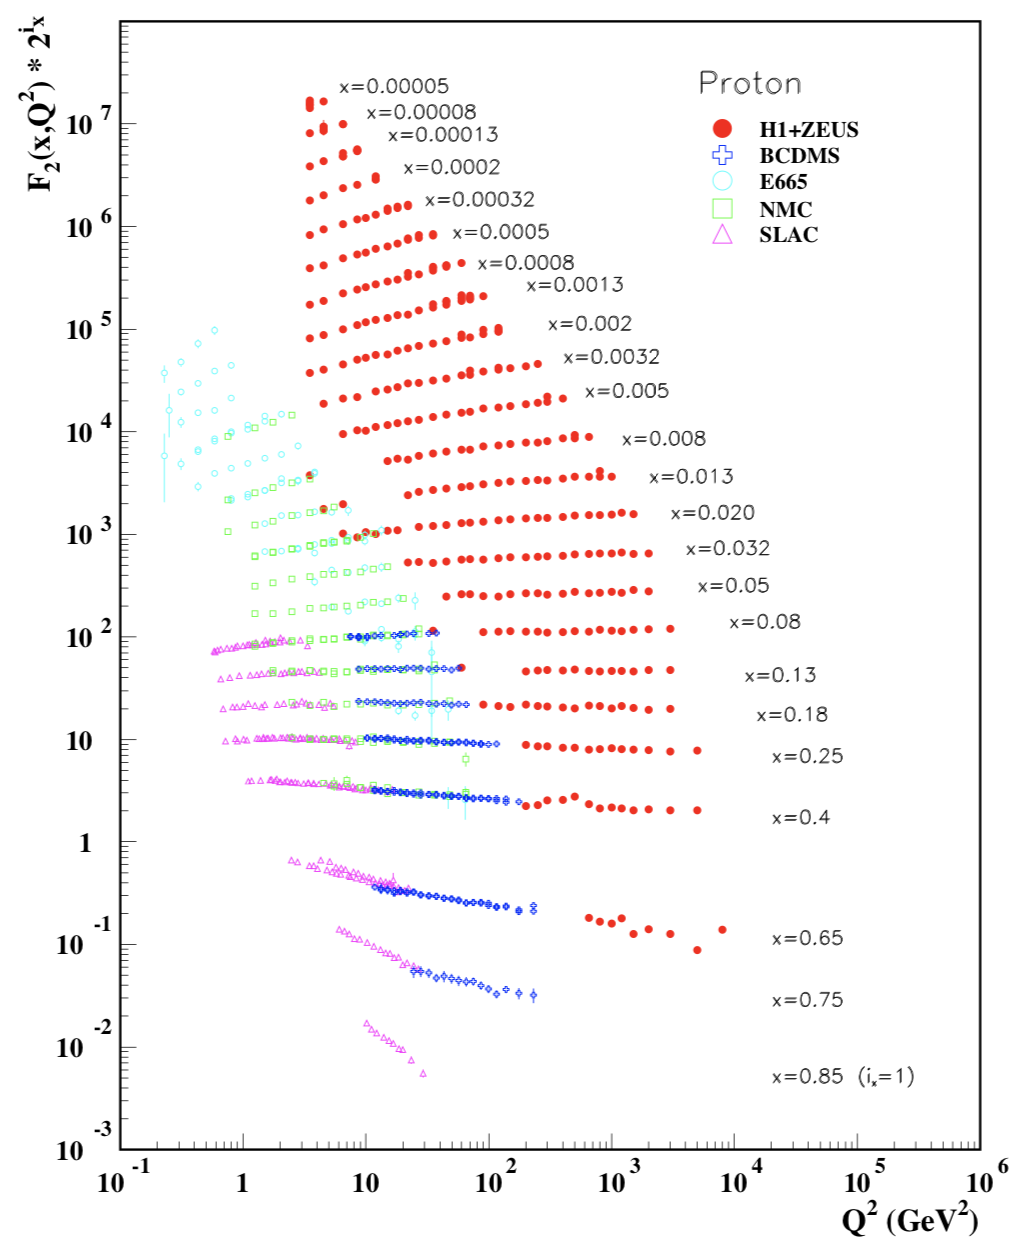
\includegraphics[scale=0.65]{./gfx/F2.png}
	\caption{The proton structure function $F^2_p$ measured in electromagnetic scattering of electrons and positrons on protons (collider experiments H1 and ZEUS for $Q^2 \geq$ 2 GeV$^2$), in the kinematic domain of the HERA data, and for electrons (SLAC) and muons (BCDMS, E665, NMC) on a fixed target. Figure taken from \cite{PDG}.}
	\label{pic:F2}
\end{figure}

\subsection{QCD-improved QPM}

The $Q^2$ dependence observed in previous subsection can be estimated by introducing the quark interaction from QCD.
Quantum ChromoDynamics is a non-abelian gauge theory based on a symmetry group SU(3) which describes the strong interaction.
The charge of this theory is called colour and the force carriers are the gluons, which are also coloured particles. The
internal nucleon dynamic is dominated by the gluon emission and absorption by the 3 valence quarks. The gluons can create
pairs of quark-antiquark or emit gluons. This creates a cloud of gluons and virtual $q\bar{q}$ pairs known as sea quarks.

The QCD coupling constant $\alpha_s$ depends on the scale of the interaction. At low energies quarks or gluons are always
forming colorless particles as hadrons : this is the confinement. At high energies quarks or gluons are free particles :
this is asymptotic freedom.

Depending on the energy regime, a process can be labeled as a hard ($\alpha \sim 0$) or soft process ($\alpha \approx 0$).
Hard processes can be described within the perturbative QCD (pQCD) framework when soft processes can only be parametrized
from experimental data. This two regimes differ by the factorisation scale $\Lambda$. As in DIS the scale variable is $Q^2$,
the DIS cross-section can only be factorized in terms of soft and hard processes at $Q^2>1$GeV$^2$ : the hard process is the
lepton-quark interaction $\sigma_q$ and the soft process is a non-calculable universal quantity which are the PDFs.

The resolution of the virtual photon probe is proportional to $1/Q^2$ (Fig. \ref{pic:Q2res}). At $Q^2 \approx 0$, the virtual photon sees the
nucleon as a point-like particle. As $Q^2$ increases, the virtual starts to interact with the nucleons constituents. At large $Q^2$
the virtual photon is able to access the gluons. The first QCD correction to the QPM concerns the gluon emission by the initial and
the final quark. The splitting functions $P_{ij}(x/\xi)$ are the probability that a quark or gluon of type $j$ and momentum fraction
$\xi$ is the parent of i with momentum fraction $x$.

\begin{figure}[!h]
  \centering
	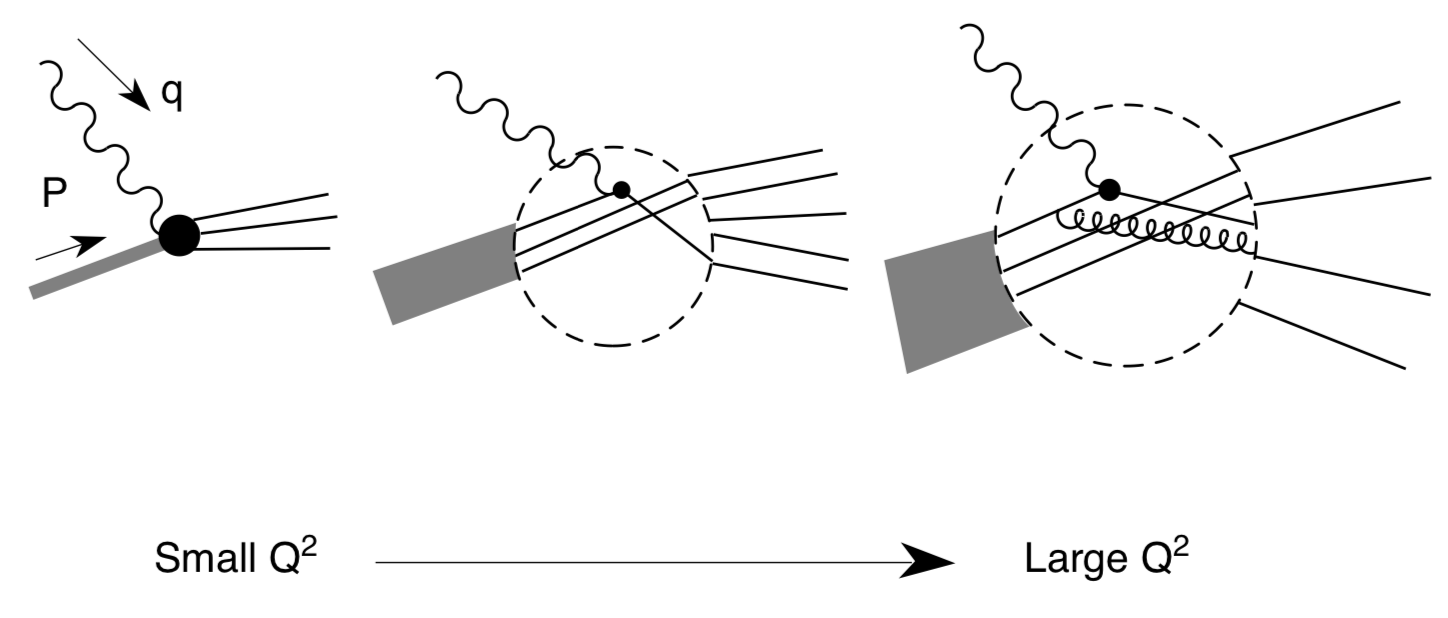
\includegraphics[scale=0.6]{./gfx/Q2res.png}
	\caption{Resolution of the photon probe versus $Q^2$.}
	\label{pic:Q2res}
\end{figure}

The $Q^2$ dependence is calculated by the Dokshiter-Gribov-Lipatov-Altarelli-Parisi (DGLAP) equations.

\begin{equation}
  \frac{dq_i(x,Q^2)}{dlnQ^2} = \frac{\alpha_s(Q^2)}{2\pi}\sum\limits_{j}\int_{x}^{1}P_{ij}(x/\xi,\alpha_s(Q^2))q_i(\xi,Q^2)
\end{equation}

If the PDFs are known at a given scale $Q_0^2$, they can be evolved to any given $Q^2$ using these equations.

%----------------------------------------------------------------------------------------

\section{Determination of Parton Distribution Functions}

The PDFs are non-perturbative quantities and thus cannot be devised from a theoretical framework. A global fit to world data is the
only way to quantify them. This global fit is only possible because PDFs are universal quantities, ie. they are process independent.
The world data consists of lepton-nucleon DIS, collider experiments ($pp$ or $p\bar{p}$), neutrino scattering, etc. As experiments
cover different kinematic ranges, this allow one to determine the PDFs in a large ($x$,$Q^2$) space.

For the fit to be performed, a functional form has to be provided at $Q^2_0$. They are usually following the form : $xq_i(x,Q^2_0) = x^{\alpha}(1-x)^{\beta}$
with following terms refining the fit, reaching a number of free parameters from 10 to 25. The DGLAP equations are then used to evolve
the PDFs to a given $Q^2$. An example of a fit done by the MMHT group at Next to Leading Order (NLO) for different $Q^2$ values is shown in Fig. \ref{fig:MMHT}.

\begin{figure}[htb!]
\centerline{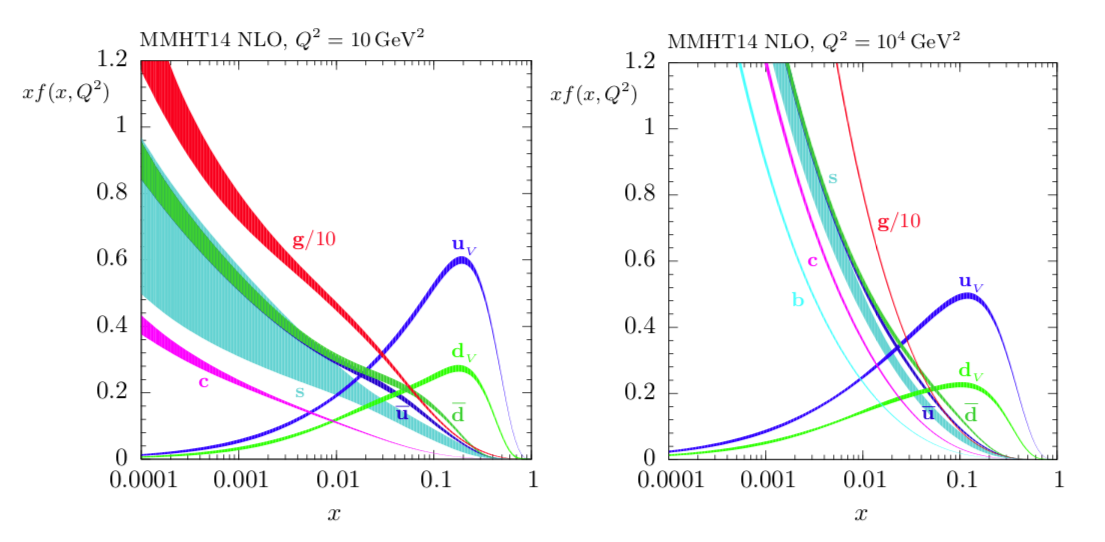
\epsfig{file=gfx/MMHT.png,width=14cm}}
\caption{Unpolarized PDFs at Next to Leading Order (NLO) from MMHT group at $Q^2$ = 10 GeV$^2$ (left) and $Q^2$ = 10$^4$ GeV$^2$ (right) with associated 68\%
confidence-level uncertainty bands. Figure taken from \cite{MMHT}.}\label{fig:MMHT}
\end{figure}

%----------------------------------------------------------------------------------------

\section{Semi-Inclusive Deep Inelastic Scattering}

As its name induces, Semi-Inclusive Deep Inelastic Scattering (SIDIS) is the semi-inclusive channel of the overall DIS process. In the
final state, a hadron and the scattered lepton are detected ($l+N \rightarrow l'+h+X$) and a new invariant variable $z$ is introduced,
which corresponds to the energy fraction of the virtual photon held by the hadron $h$ (Eq. \ref{eq:SIDIS}).

\begin{equation}
  z = \frac{\textbf{P}\cdot\textbf{p}_h}{\textbf{P}\cdot\textbf{q}} \stackrel{lab}{=} \frac{E_h}{\nu}
  \label{eq:SIDIS}
\end{equation}

The semi-inclusive cross section reads \cite{SIDISXS}:

\begin{equation}
  \frac{d\sigma}{dxdydz} \stackrel{QPM}{=} \frac{8\pi\alpha^2ME}{Q^4}\left[xy^2H_1(x,Q^2,z)+(1-y)H_2(x,Q^2,z)\right]
  \label{eq:SIDISXS}
\end{equation}

where $H_1$ and $H_2$ are structure functions related to $F_1$ and $F_2$ \cite{SF} :

\begin{equation}
  \sum\limits_{h}\int_{0}^{1} H_i(x,Q^2,z)dz = F_i(x,Q^2), i \in  \llbracket1,2\rrbracket
\end{equation}

Other variables can be used to describe the hadron in SIDIS (Table. \ref{tab:SIDIS}).

\begin{table}[h!]
  \caption{SIDIS kinematic variables.}
  \label{tab:SIDIS}
  \begin{tabularx}{\textwidth}{r|lX}
    \hline
    \hline
    Variable & Description \\
    \hline
    \hline
    $\textbf{p}=(E_h,\vec{p}_h)$ & Hadron 4-momentum vector \\
    $p_{h\|}$ & Component of $\vec{p}_h$ along $\vec{q}$ \\
    $p_{h\bot}$ & Transverse component of $\vec{p}_h$ with respect to $\vec{q}$ \\
    $\theta_h$ & Angle between $\vec{q}$ and $\vec{p}_h$ \\
    $\Phi_h$ & Angle between the scattering plane and the hadron production plane \\
    $z$ & Energy fraction of the virtual photon transferred to the hadron $h$ \\
    \hline
    \hline
  \end{tabularx}
\end{table}

\subsection{SIDIS in QPM}

The factorization theorem allows to describe the hadron production as two independent processes : the hard process $\sigma_q$
describing the absorption of the virtual photon $\gamma^*$ by the quark $q$ and the soft process $D_q^h(z)$ ruling the
fragmentation of the quark $q$ into a hadron $h$.

\begin{figure}[!h]
  \centering
	% 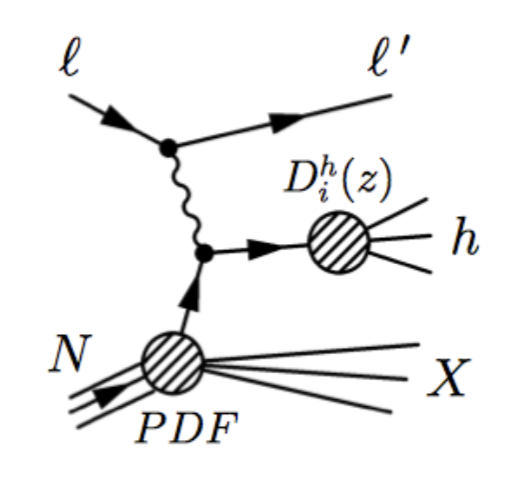
\includegraphics[scale=0.6]{./gfx/SIDIS.png}
  \begin{tikzpicture} \begin{feynman}
  \vertex (i1) {\(l\)};
  \vertex[right=2cm of i1] (a);
  \vertex[above right=2cm of a] (i2) {\(l'\)};
  \vertex[blob,below=2cm of a] (b) {};
  \vertex[blob,below left=2cm of b] (c) {\(q(x)\)};
  \vertex[below left=2cm of c] (f12) {\(N\)};
  \vertex[right=2cm of c] (f22);
  \vertex[below=0.3cm of f22] (f23);
  \vertex[above=0.3cm of f22] (f21);
  \vertex[blob, right=of b] (d) {\(D^h_q(z)\)};
  \vertex[above right=of d] (d1) {\(h^{\pm}\)};
  \vertex[right=of d] (d2) {\(\pi^{\pm}\)};
  \vertex[below right=of d] (d3) {\(K^{\pm}\)};

  \diagram* { (i1) -- [fermion] (a) -- [fermion] (i2),
  (a) -- [photon, edge label=\(\gamma^*\)] (b) [blob],
  (c) [blob] -- [fermion] (b) [blob],
  (b) [blob] -- [fermion] (d) [blob],
  (f12) -- [double distance=7pt] (c) [blob] -- [plain] (f22),
  (f12) -- [fermion] (c) [blob],
  (c) [blob] -- [plain] (f21),
  (c) [blob] -- [plain] (f23),
  (d) [blob] -- [plain] (d1),
  (d) [blob] -- [plain] (d2),
  (d) [blob] -- [plain] (d3),
  };
  \draw [decoration={brace}, decorate] (f21.north east) -- (f23.south east) node [pos=0.5, right] {\(X\)};
  \end{feynman} \end{tikzpicture}
	\caption{Factorization in semi-inclusive deep inelastic scattering.}
	\label{pic:SIDIS}
\end{figure}

The structure functions $H_i(x,Q^2,z)$ contain the information on what happens to the struck quark after the interaction with the virtual photon. The fragmentation function (FF) $D_q^h(z,Q^2)$ is defined as the probability for a quark of flavour $q$ to fragment into a hadron $h$ with a fraction of energy $z$. The expression of the SIDIS cross section can be expressed at LO in terms of the PDFs and the FFs \cite{SIDISPDFFF} :

\begin{equation}
  \frac{d^3 \sigma^{unpolarized}}{dxdydz} \stackrel{LO}{=} \frac{8\pi\alpha^2ME}{Q^2}\left[\frac{1}{2}y^2+(1-y-\frac{y^2 \gamma^2}{4})\right]x\sum\limits_qe^2_qq(x)D_q^h(z)
  \label{eq:unpolSIDIS}
\end{equation}

\subsection{Scaling and $Q^2$ evolution}

A scaling violation is observed for the FFs extracted from $e^+e^-$ annihilation \cite{SIAFF}. The scaling is present in the $x = 2p_h/\sqrt{s}$
bin 0.1-0.2. At low x ($x$ < 0.1) the FFs increases with $\sqrt{s}$, while at large $x$, the FFs are shifted towards lower values for large
$Q^2$.

\begin{figure}[!h]
  \centering
	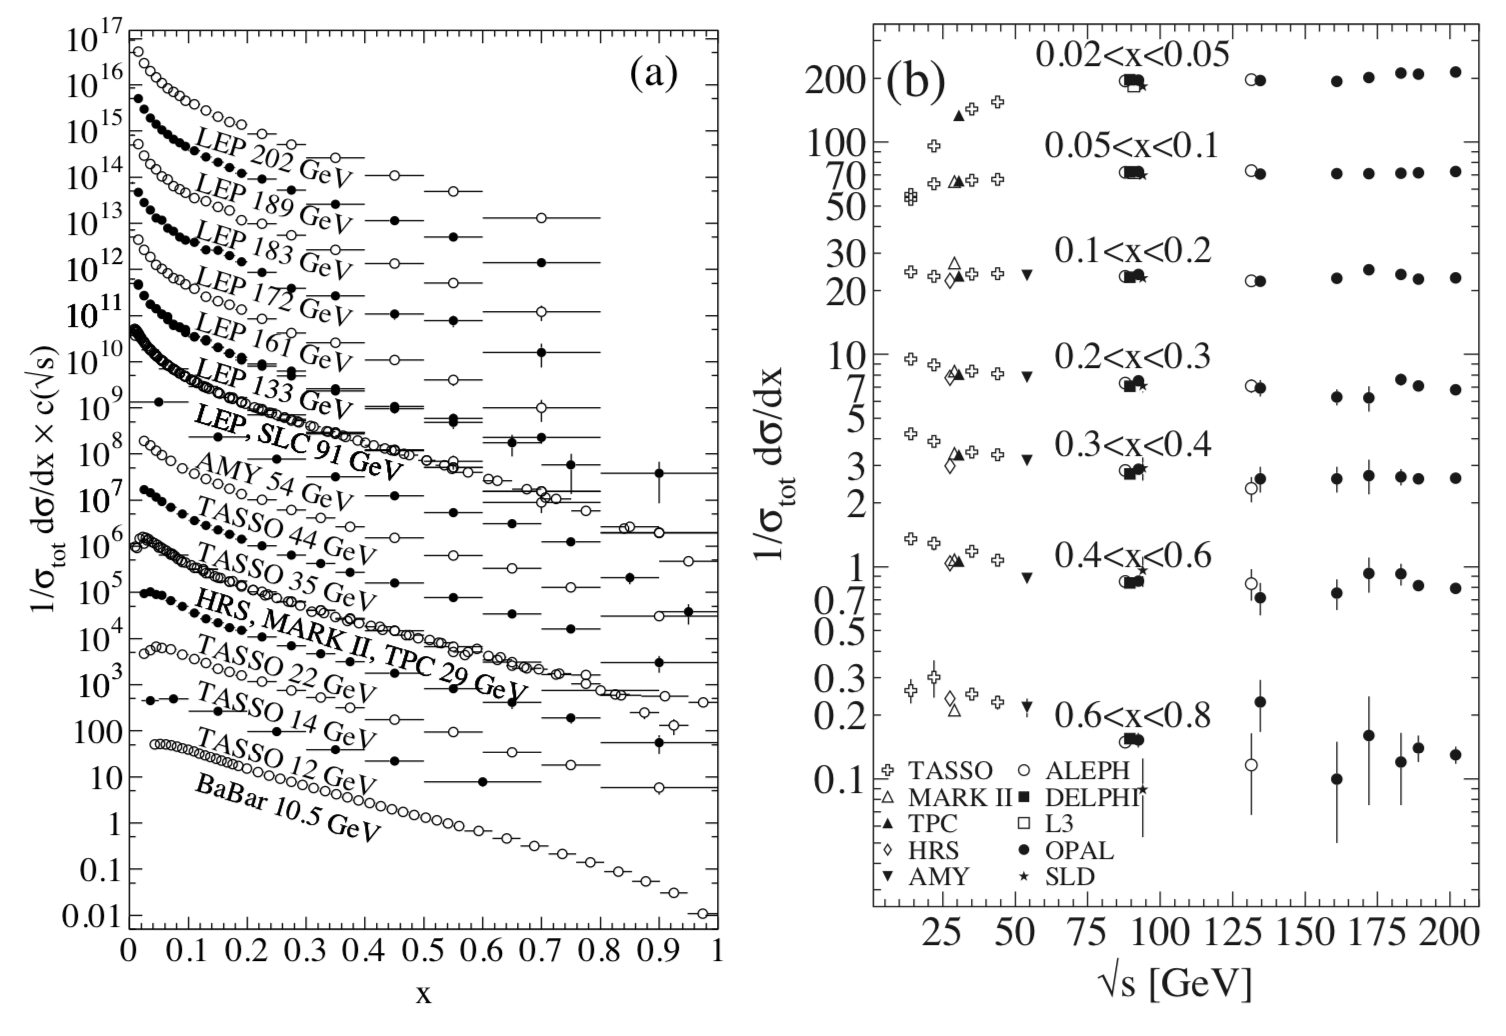
\includegraphics[scale=0.6]{./gfx/FFscale.png}
	\caption{The $e^+ e^-$ fragmentation function for all charged particles for different center of mass energy $\sqrt{s}$ versus $x$ (a) and for various range of $x$ versus $\sqrt{s}$. Figures taken from \cite{PDG}.}
	\label{pic:FFscale}
\end{figure}

The evolution of the fragmentation functions is done with the DGLAP equations \cite{DGLAP} :

\begin{equation}
  \frac{dD_q^h(z,Q^2)}{dlnQ^2} = \frac{\alpha_s(Q^2)}{2\pi}\sum\limits_j\int_{x}^{1}P_{qj}\left(z/\xi,\alpha_s(Q^2)\right)D_q^h(\xi,Q^2)\frac{d\xi}{\xi}
\end{equation}

In Fig. \ref{pic:QuarkFrag} is shown the fragmentation of quark and gluons. Four different fragmentation channel can be separated : the fragmentation of a quark $q_i$ through its own decay after emmiting a gluon G ($P_{qq}D_{q_i}^h$), through the decay of a gluon G ($P_{Gq}D_{G}^h$), the fragmentation of a gluon splitting into a quark-antiquark pair and following hadronization of the quark in hadron ($P_{qG}D_{q_i}^h$) and eventually the gluon fragmentation via the three-gluon self-interaction ($P_{GG}D_{G}^h$).

\begin{figure}[!h]
  \centering
	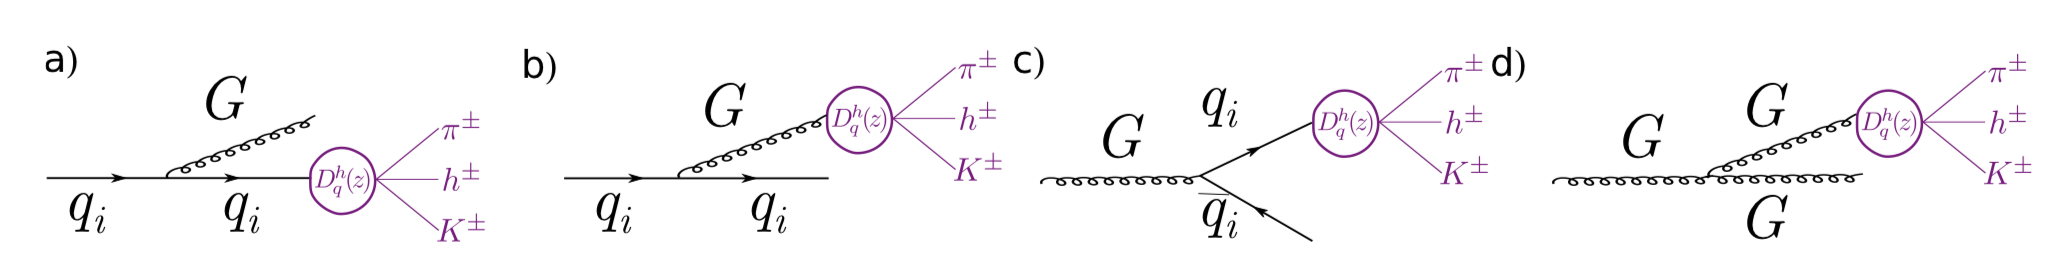
\includegraphics[scale=0.45]{./gfx/QuarkFrag.png}
	\caption{The fragmentation of the quark $q_i$ decaying into a hadron $h$ while emitting a gluon $G$ ($P_{qq}D^h_{q_{i}}$) (a), the fragmentation of the quark $q_i$ through a gluon $G$ ($P_{Gq}D^h_{G}$) (b), the fragmentation of the gluon $G$ via the creation of a $q_i \bar{q_i}$ pair and the decay of $q_i$ ($P_{qG}D^h_{q_{i}}$) (c) and the fragmentation of the gluon $G$ via a three gluon vertex ($P_{GG}D^h_{G}$) (d)}
	\label{pic:QuarkFrag}
\end{figure}

%----------------------------------------------------------------------------------------

\section{Fragmentation Functions}\label{sec:FF}

When computing the cross-section of a given process $A+B \rightarrow h+X$, this cross-section is found to be a convolution of three different terms (Eq. \ref{eq:facto}) : one non-perturbative term involving the PDFs (probability to obtain parton $a$ from nucleus $A$ $f_{a/A}(x_a,Q^2)$), one matrix element term for perturbative calculation ($d\sigma_{a,b \rightarrow c}(x_a,x_b,Q^2)$) and a last non-perturbative term involving the FFs (probability to obtain hadron $h$ from parton $c$ $D^h_c(x_c,Q^2)$). The FFs describes the hadronization ie. the quark fragmentation into a hadron. This is a non-perturbative term as the hadronization is a soft process.

\begin{equation}
  d\sigma_{A+B \rightarrow h+X} = \sum_{a,b,c} \left[ f_{a/A}(x_a,Q^2) f_{b/B}(x_b,Q^2) \right] \otimes \left[ d\sigma_{a,b \rightarrow c}(x_a,x_b,Q^2) \right] \otimes \left[ D^h_c(x_c,Q^2) \right]
  \label{eq:facto}
\end{equation}

Different models have been developed to describe how quarks confine together to make a hadron.

\subsection{Lund String Fragmentation Model}

In the Lund String Model \cite{LUND}, the hadron production is explained by the creation of quark-antiquark pairs $q\bar{q}$. The strong interaction between partons is represented by a string. The energy inside the string is linear function of the distance between two stringed partons. At some point the energy is large enough to create a new $q\bar{q}$ pair and the string breaks. Each paired remnants have new strings and the process repeats until there are only hadrons. The hadronization scheme in the Lund model in the center of mass frame is illustrated in Fig. \ref{pic:Lund}. The virtual photon is absorbed by the $u$ quark and in consequence the $u$ quark is ejected from the nucleon. The remaining $u$ quark bounds with the $\bar{d}$ quark to form a $\pi^+$ with a given $z$. The remaining system repeats fragmentation process until the energy is smaller than the available energy $\nu$.

\begin{figure}[!h]
  \centering
	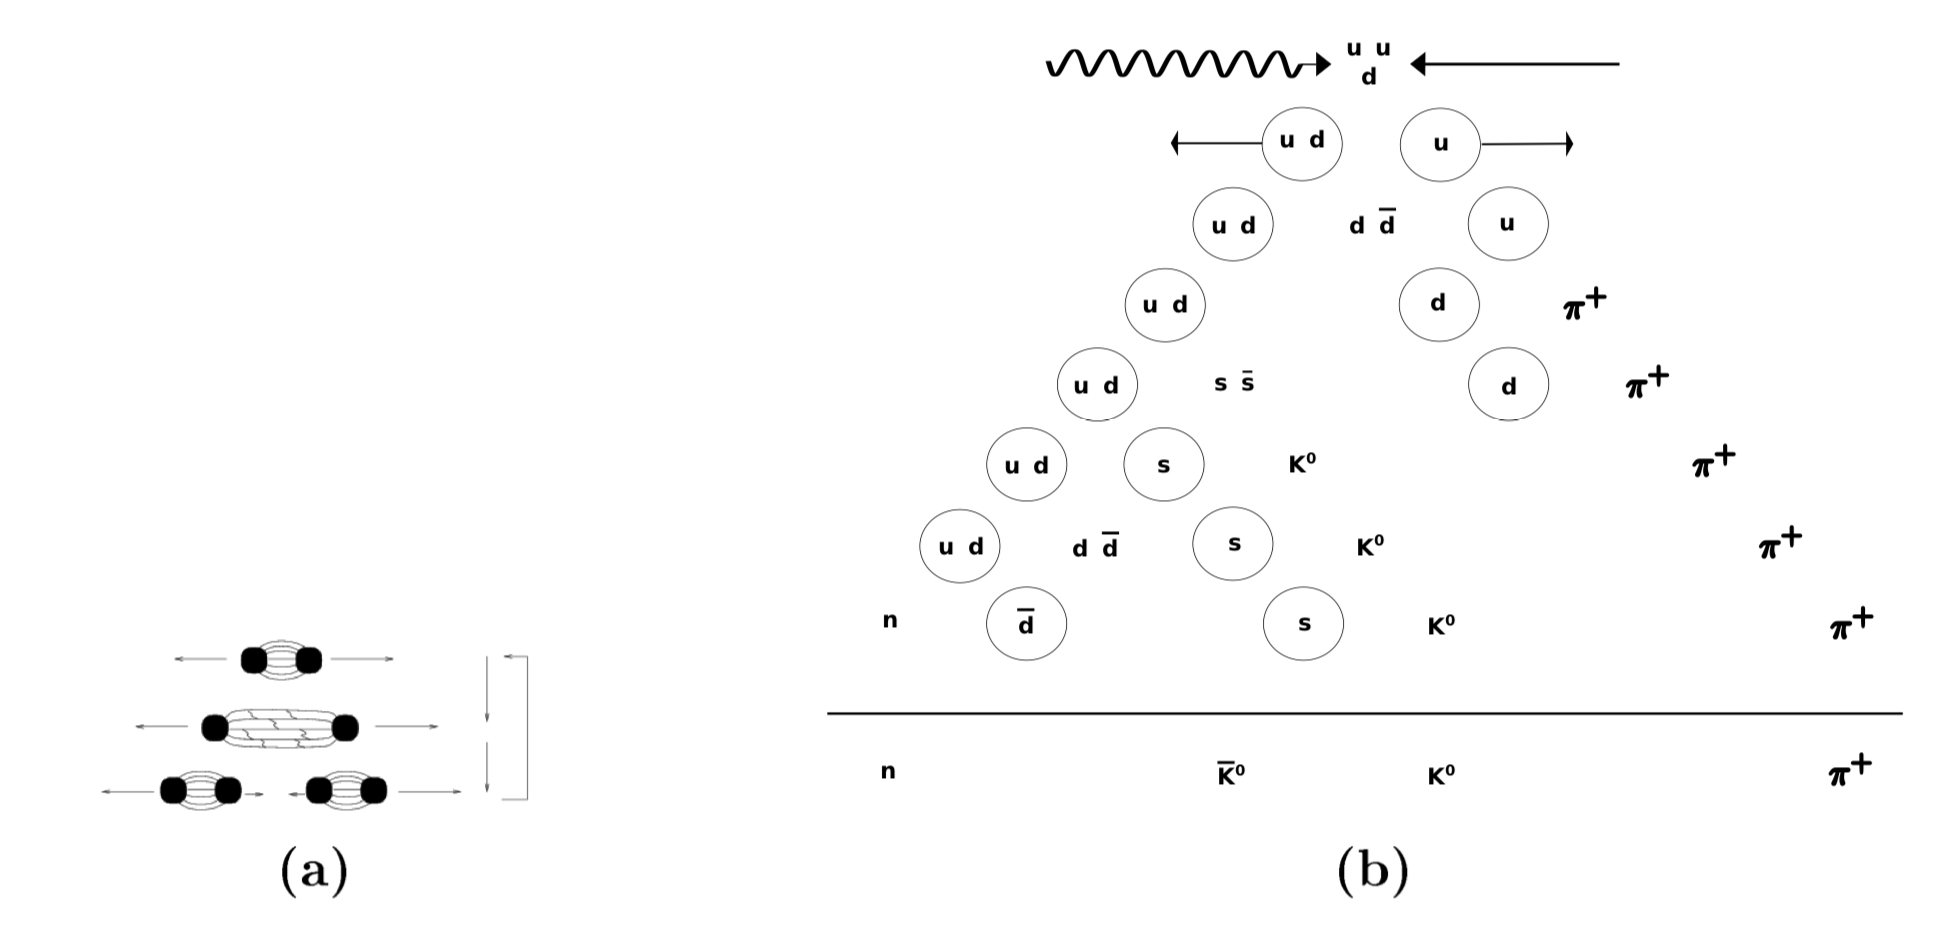
\includegraphics[scale=0.45]{./gfx/Lund.png}
	\caption{The fragmentation process in the Lund model.}
	\label{pic:Lund}
\end{figure}

\subsection{Quark Fragmentation Regions}

At this point only the production from struck quarks were considered. Nevertheless, it is also possible that a spectator quark which is not involved in the scattering process fragments into hadrons. This phenomenon is happening in two well $p_h$-defined regions : the target fragmentation region where the final hadron $h$ has a small momentum in the rest frame of the target and the current fragmentation region where the product $\textbf{P}\cdot\textbf{p}_h$ grows with $Q^2$. This hadron production can contaminate the hadron production from the actual SIDIS process. To deal with this issue, Berger \cite{BERGER} came with a criterion based on the rapidity of the final state $\eta$. The sign of $\eta$ is linked to the different regions : if $\eta$ > 0 the hadron moves towards the direction of the virtual photon and is a current hadron, else is $\eta$ < 0 the hadron is a target remnant (Fig. \ref{pic:Berger}). As the typical hadronic correlation length in rapidity is $\delta \sim 2$, a separation criterion, the Berger criterion, is that $\Delta\eta = \eta_{max}-\eta_{min} \geq 2\delta$ or in terms of DIS kinematics variables $W \gtrsim 7.4$ GeV. It is important to be able to separate the current and target fragmentation to ensure the quark fragmentation into hadrons is independent of the production of the quark.

\begin{figure}[!h]
  \centering
	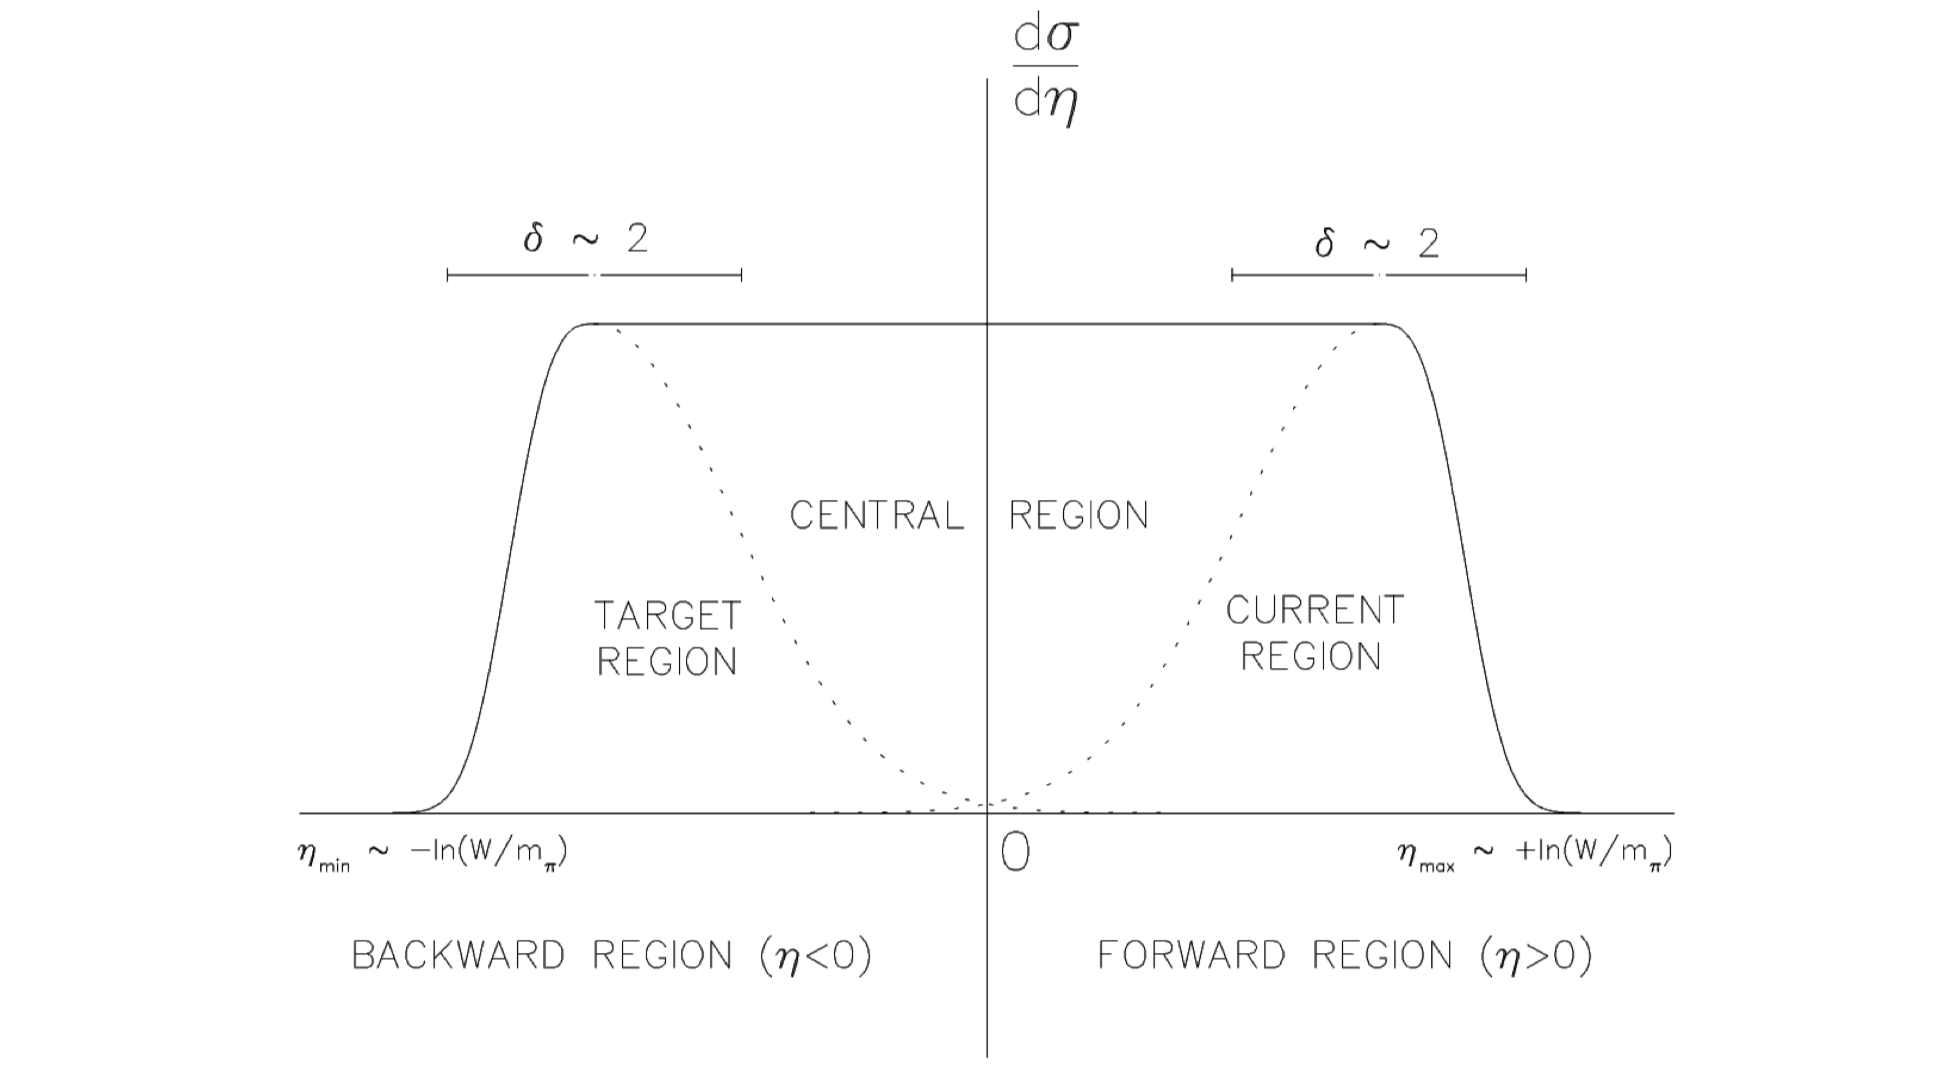
\includegraphics[scale=0.5]{./gfx/Berger.png}
	\caption{Typical hadronic rapidity ($\eta$) distribution.}
	\label{pic:Berger}
\end{figure}

\subsection{Fragmentation Function Symmetries}

A FF $D^h_q(z,Q^2)$ is existing for any flavour q and hadron h. Considering only the light quark ($u$,$\bar{u}$,$d$,$\bar{d}$,$s$ and $\bar{s}$) as the mass
threshold for heavy quarks is higher than the covered kinematic domain, it implies that for charged hadrons one has to measure twelve different fragmentation
functions, evenly spread between positive and negative hadrons. Nevertheless, within the QCD-improved QPM, symmetries as isospin or charge-conjugation can be
used to reduce the number of independent fragmentation functions to measure.

The FFs can be splitted into two main categories. If a valence quark fragments into a hadron h, the FF is said to be favoured ($D^h_{fav}$), while for a sea quark the FF is unfavoured ($D^h_{unf}$).

Concerning the pions, the charge-conjugation symmetry reduces the number of independent fragmentation functions to six. The application of the isospin symmetry (viz. $D^{\pi^+}_u = D^{\pi^+}_{\bar{u}}$ for $\pi^+$) lowers this number to two :

\begin{equation}
  \begin{split}
    D^h_{fav} : D^{\pi^+}_u = D^{\pi^-}_{\bar{u}}, D^{\pi^-}_d = D^{\pi^+}_{\bar{d}} \\
    D^h_{unf} : D^{\pi^-}_u = D^{\pi^+}_{\bar{u}}, D^{\pi^+}_d = D^{\pi^-}_{\bar{d}}, D^{\pi^{\pm}}_s = D^{\pi^{\mp}}_{\bar{s}}
  \end{split}
\end{equation}

Concerning the kaons, only the charge-conjugation symmetry can be applied, reducing the number of independent fragmentation functions to six. Nevertheless, other assumptions can be made to further reduce this number. One of them is to consider three categories of FFs : the favoured, grouping the FF of valence quarks $u$ and $\bar{u}$, the strange, grouping the FF of the strange quarks and the unfavoured, grouping the rest :

\begin{equation}
  \begin{split}
    D^h_{fav} : D^{K^+}_u = D^{K^-}_{\bar{u}} \\
    D^h_{str} : D^{K^+}_{\bar{s}} = D^{K^-}_{s} \\
    D^h_{unf} : D^{K^+}_{\bar{u}} = D^{K^-}_{u}, D^{K^+}_s = D^{K^-}_{\bar{s}}, D^{K^{\pm}}_{d} = D^{K^{\mp}}_{\bar{d}}
  \end{split}
\end{equation}

%----------------------------------------------------------------------------------------

\section{State of the art of the fragmentation functions}

\subsection{Measurements}

The production of hadrons from the QCD parton model is hard to compute as hadron mass can be smaller than $\Lambda_{QCD}$. In order to overcome this limitation, measurement of hadron production at different collision energies are made. As the factorisation theorem is valid and the FFs universal (experimentally tested by Kniehl, Kramer and Pötter \cite{Universality}), global fit of FFs on world data can be made.
Three different processes are so far used to extract quark fragmentation functions : electron-positron annihilation (SIA), lepton-nucleon SIDIS and hadron-hadron collisions ($pp$ or $p\bar{p}$). The SIA data (LEP\cite{LEP}, SLAC\cite{SLAC}, BaBar\cite{BABAR} and BELLE\cite{BELLE}) provide on one hand the cleanest access to the FFs since the cross-section of the process does not involve PDFs and are well understood with calculations available to NNLO, but on the other hand they are not able to separate $D^h_q$ and $D^h_{\bar{q}}$ and have a limited access to gluon FF $D^h_g$. The data from hadron-hadron collisions (UA5\cite{UA5}, UA1\cite{UA1}, ALICE\cite{ALICE}, CMS\cite{CMS}, ATLAS\cite{ATLAS}, RHIC\cite{RHIC}) give access to $D^h_q$, $D^h_{\bar{q}}$ and $D^h_g$ but allow no direct access to $z$ and theory is not yet under control.

Concerning the data from SIDIS processes, they can be compared to data from previously presented processes if they all belong to the current fragmentation region (see Section \ref{sec:FF}). The SIDIS data have the advantages that the factorization has been proven to all orders of $\alpha_s$ and to cover a wider range in $Q^2$ compared to SIA as measurement are done at a much lower scale. The experiments providing inputs for the SIDIS process are EMC\cite{EMC} (muon beam, proton/deuteron target), E00-108\cite{E00108} (electron beam, proton/deuteron target), HERMES\cite{HERMES} (electron beam, proton/deuteron target) and COMPASS (electron beam, proton/deuteron target, only deuteron data published so far\cite{COMPASS2006}).

A summary of the aspects of the different processes can be found in Table\ref{tab:FFProcesses}.

\begin{table}[!h]
  \caption{Fragmentation functions access for different processes.}
  \label{tab:FFProcesses}
  \centering
  \begin{tabular}{cccc}
    \hline
    \hline
    & $e^+ e^- annihilation$ & $pp$/$p\bar{p}$ collision & SIDIS \\
    \hline
     &   \resizebox{3cm}{3.5cm}{\begin{tikzpicture} \begin{feynman}
     \vertex (i1) {\(e^{-}\)};
     \vertex[right=2cm of i1] (a);
     \vertex[above right=2cm of a] (i2) {\(e^{+}\)};
     \vertex[blob,below=2cm of a] (b) {\(\widehat{\sigma_q}\)};
     \vertex[below left=2cm of b] (f12);
     \vertex[below=0.3cm of f12] (f13);
     \vertex[above=0.3cm of f12] (f11);
     \vertex[blob,below right=2cm of b] (d) {\(D^h_q(z)\)};
     \vertex[above right=of d] (d1) {\(h^{\pm}\)};
     \vertex[right=of d] (d2) {\(\pi^{\pm}\)};
     \vertex[below right=of d] (d3) {\(K^{\pm}\)};

     \diagram* { (i1) -- [fermion] (a) -- [anti fermion] (i2),
     (a) -- [photon, edge label=\(\gamma^{*}/Z^{0}\)] (b) [blob],
     (f12) -- [plain] (b) [blob] -- [fermion] (d) [blob],
     (f13) -- [plain] (b) [blob],
     (f11) -- [plain] (b) [blob],
     (d) [blob] -- [plain] (d1),
     (d) [blob] -- [plain] (d2),
     (d) [blob] -- [plain] (d3),
     };
     \draw [decoration={brace}, decorate] (f13.south west) -- (f11.north west) node [pos=0.5, left] {\(X\)};
   \end{feynman} \end{tikzpicture}}
      & \resizebox{3.5cm}{3cm}{\begin{tikzpicture} \begin{feynman}
    \vertex (i1) {\(p\)};
    \vertex[blob,right=2cm of i1] (a) {\(q(x)\)};
    \vertex[below=6cm of i1] (i2) {\(p/\bar{p}\)};
    \vertex[blob,right=2cm of i2] (b) {\(q(x)\)};
    \vertex[blob,below right=4cm of a] (c) {\(\widehat{\sigma}_q\)};
    \vertex[above right=of c] (f1);
    \vertex[blob, below right=of c] (d) {\(D^h_q(z)\)};
    \vertex[above right=of d] (d1) {\(h^{\pm}\)};
    \vertex[right=of d] (d2) {\(\pi^{\pm}\)};
    \vertex[below right=of d] (d3) {\(K^{\pm}\)};

    \diagram* { (i1) -- [double distance=7pt] (a) [blob], (i1) -- [fermion] (a) [blob],
    (i2) -- [double distance=7pt] (b) [blob], (i2) -- [fermion] (b) [blob],
    (a) -- [fermion] (c) [blob], (b) -- [fermion] (c) [blob], (c) [blob] -- [fermion] (f1), (c) [blob] -- [fermion, edge label=\(q\)] (d) [blob],
    (d) [blob] -- [plain] (d1),
    (d) [blob] -- [plain] (d2),
    (d) [blob] -- [plain] (d3),
    };
    \end{feynman} \end{tikzpicture}}
      & \resizebox{3cm}{3.5cm}{\begin{tikzpicture} \begin{feynman}
      \vertex (i1) {\(l\)};
      \vertex[right=2cm of i1] (a);
      \vertex[above right=2cm of a] (i2) {\(l'\)};
      \vertex[blob,below=2cm of a] (b) {\(\widehat{\sigma}_q\)};
      \vertex[blob,below left=2cm of b] (c) {\(q(x)\)};
      \vertex[below left=2cm of c] (f12) {\(N\)};
      \vertex[right=2cm of c] (f22);
      \vertex[below=0.3cm of f22] (f23);
      \vertex[above=0.3cm of f22] (f21);
      \vertex[blob, right=of b] (d) {\(D^h_q(z)\)};
      \vertex[above right=of d] (d1) {\(h^{\pm}\)};
      \vertex[right=of d] (d2) {\(\pi^{\pm}\)};
      \vertex[below right=of d] (d3) {\(K^{\pm}\)};

      \diagram* { (i1) -- [fermion] (a) -- [fermion] (i2),
      (a) -- [photon, edge label=\(\gamma^*\)] (b) [blob],
      (c) [blob] -- [fermion] (b) [blob],
      (b) [blob] -- [fermion] (d) [blob],
      (f12) -- [double distance=7pt] (c) [blob] -- [plain] (f22),
      (f12) -- [fermion] (c) [blob],
      (c) [blob] -- [plain] (f21),
      (c) [blob] -- [plain] (f23),
      (d) [blob] -- [plain] (d1),
      (d) [blob] -- [plain] (d2),
      (d) [blob] -- [plain] (d3),
      };
      \draw [decoration={brace}, decorate] (f21.north east) -- (f23.south east) node [pos=0.5, right] {\(X\)};
    \end{feynman} \end{tikzpicture}}\\
    Dependence & $\widehat{\sigma} \otimes FF$ & $\widehat{\sigma} \otimes PDF \otimes PDF \otimes FF$ & $\widehat{\sigma} \otimes PDF \otimes FF$ \\
    Access $D^h_{q}$ and $D^h_{\bar{q}}$ & \ding{55} & \ding{51} & \ding{51} \\
    Access parton kinematics & \ding{51} & \ding{55} & \ding{51} \\
    Theoretical calculation & LO, NLO, NNLO & LO, NLO & LO, NLO \\
    \hline
  \end{tabular}
\end{table}

\subsection{Accessing the fragmentation functions in SIDIS}

The hadron multiplicities is a convenient way in SIDIS to access the FFs. They are defined as the averaged number of hadrons produces per DIS events defined by :

\begin{equation}
  M^h(x,Q^2,z) = \frac{d\sigma^{lN \rightarrow l'hX}}{d\sigma^{lN \rightarrow l'X}dz}
\end{equation}

Remembering the expressions of the DIS and SIDIS cross-sections from Eqs. \ref{eq:unpolDIS} and \ref{eq:unpolSIDIS}, one can obtain :

\begin{equation}
  M^h(x,Q^2,z) = \frac{\sum_q e^2_q q(x,Q^2) \otimes D^h_q(z,Q^2)}{\sum_q e^2_q q(x,Q^2)} \stackrel{LO}{=} \frac{\sum_q e^2_q q(x,Q^2) D^h_q(z,Q^2)}{\sum_q e^2_q q(x,Q^2)}
\end{equation}

As PDFs and FFs depend on different variables $x$ and $z$ allows to go from a convolution to a single product. By measuring $M^h(x,Q^2,z)$ for positive and negative hadrons, one can distinguish $D^h_q$ and $D^h_{\bar{q}}$. The procedure of FFs extraction from COMPASS multiplicities measurement is given in Chapter \ref{ch:FF}.

\subsection{Global fits of multiplicities data and parametrizations of FFs}

As the FFs are universal quantities, a global QCD fit of available data on multiplicities from SIA, SIDIS and $pp$/$p\bar{p}$ collisions can be performed to give a general parametrization of the FFs. Some parametrizations are only based on SIA data : Kniehl-Kramer-Poter (KKP) \cite{KKP}, Kretzer (KRE) \cite{KRE} and Hirai-Kumano-Nagai-Sudoh (HKNS) \cite{HKNS}, when the Albino-Kniehl-Kramer (AKK) \cite{AKK} parametrization uses in addition some hadron-hadron scattering data. Some only uses SIDIS data : Leader-Sidorov-Stamenov (LSS) \cite{LSS}. The newest parametrizations from de Florian-Sassot-Epele-Hernandez Pinto-Stratmann (DSEHS) \cite{DSEHS} and Sato et al. (Jefferson Lab Angular Momentum, JAM) \cite{JAM} includes all three types of data for DSEHS and SIA+SIDIS for JAM. Each parametrization has its own set of assumptions on the symmetries and its own parametrization of the $D^h_q$. A summary of the parametrization can be found in Table \ref{tab:FFParametrization}. Only DSEHS and JAM will be described more thoroughly in the following as they are the newest one (or updated recently).

\begin{table}[!h]
  \caption{Parametrization of FFs for pions and kaons.}
  \label{tab:FFParametrization}
  \centering
  \begin{tabular}{ccccccc}
    \hline
    \hline
    Parametrization & Year & \multicolumn{3}{c}{Data} & \multicolumn{2}{c}{\# FFs fitted} \\
    \hline
     & & SIDIS & $pp$/$p\bar{p}$ & SIA & $\pi$ & $K$ \\
    KKP \cite{KKP} & 2000 & \ding{55} & \ding{55} & \ding{51} & 5 & 5 \\
    KRE \cite{KRE} & 2001 & \ding{51} & \ding{55} & \ding{51} & 2 & 3 \\
    HKNS \cite{HKNS} & 2007 & \ding{55} & \ding{55} & \ding{51} & 2 & 2 \\
    AKK \cite{AKK} & 2008 & \ding{55} & \ding{51} & \ding{51} & 3 & 5 \\
    LSS \cite{LSS} & 2014 & \ding{51} & \ding{55} & \ding{55} & 3 & 3 \\
    DSEHS \cite{DSEHS} & 2017 & \ding{51} & \ding{51} & \ding{51} & 4 & 3 \\
    JAM \cite{JAM} & 2018 & \ding{51} & \ding{55} & \ding{51} & 3 & 3 \\
    \hline
  \end{tabular}
\end{table}

\subsubsection*{DSEHS parametrization}

DSEHS (previously DSS) was the first group of fitters that determined the individual FFs for quark and antiquark and the first to try to fit data coming from three different processes alltogether.
The functional they use for $D^h_q$ is the following :

\begin{equation}
  D^h_i (z,Q_0) = \frac{N^h_i z^{\alpha^h_i}(1-z)^{\beta^h_i}\left[ 1+\gamma^h_i(1-z)^{\delta^h_i}\right]}{B\left[2+\alpha^h_i,1+\beta^h_i\right]+\gamma^h_i B\left[2+\alpha^h_i,1+\beta^h_i+\delta^h_i\right]}
  \label{eq:DSEHSparam}
\end{equation}

where $N^h_i$, $\alpha^h_i$, $\beta^h_i$, $\gamma^h_i$ and $\delta^h_i$  are the fit parameters and B is a Bernoulli polynomial. For pions the two independent FFs are related by a proportionality factor $N$. Moreover, the isospin symmetry is considered only for the unfavoured case but a slightly different normalization is used in the $q+\bar{q}$ sum ($D^{\pi^{\pm}}_{d+\bar{d}} = N_{\pi^{\pm}} D^{\pi^{\pm}}_{u+\bar{u}}$). Thus four FFs are fitted for pions. For kaons, $D^{K^+}_{u+\bar{u}}$ and $D^{K^+}_{s+\bar{s}}$ are fitted independently to account for the fact that phenomenologically it is expected that the formation of secondary $s\bar{s}$, required to form $K^+$ from a $u$, should be suppressed. Previous fit from DSS showed that $D^{K^+}_{s+\bar{s}} > D^{K^+}_{u+\bar{u}}$, highlighting this fact. For the unfavoured FFs as the data are unable to discrimate between flavours, all distributions have the same functional form : $D^{K^+}_{\bar{u}} = D^{K^+}_{s} = D^{K^+}_{d} = D^{K^+}_{\bar{d}}$.
The FFs for heavy quarks (c,b) are also considered above their $\overline{MS}$ mass thresholds.
The uncertainties are computed as in the following :

\begin{equation}
  \chi^2 =  \sum_{i=1}^{N} \left[ \left( \frac{1-\mathscr{N}_i}{\delta\mathscr{N_i}} \right) + \sum_{j=1}^{N_i} \frac{(\mathscr{N}_i T_j - E_j)^2}{\delta E^2_j} \right]
  \label{eq:DSEHSuncert}
\end{equation}

where $N$ is the number of datasets with $N_i$ points each, $E_j$ are the data points and $\delta E_j$ their error and $T_j$ the theoretical estimate for a given set. The normalisation factor $\mathscr{N}_i$ is defined as $\delta \chi^2 / \delta\mathscr{N}_i = 0$.

\begin{table}[!h]
  \caption{DSEHS FFs hypotheses for pions and kaons.}
  \label{tab:DSEHSParametrization}
  \centering
  \begin{tabular}{ll}
    \hline
    \hline
     & Pions \\
    \hline
    Favoured & $D^{\pi^{+}}_{u} = N_{\pi^{+}} D^{\pi^{+}}_{\bar{d}}$, $D^{\pi^{-}}_{d} = N_{\pi^{-}} D^{\pi^{-}}_{\bar{u}}$ \\
    Unfavoured & $D^{\pi^{+}}_{\bar{u}} = D^{\pi^{+}}_{d}$, $D^{\pi^{+}}_{\bar{s}} = D^{\pi^{+}}_{s} = N'_{\pi^{+}} D^{\pi^{+}}_{\bar{u}}$ \\
     & $D^{\pi^{-}}_{\bar{d}} = D^{\pi^{-}}_{u}$, $D^{\pi^{-}}_{\bar{s}} = D^{\pi^{-}}_{s} = N'_{\pi^{-}} D^{\pi^{-}}_{u}$ \\
    Gluons & $D^{\pi^{+}}_{g}, D^{\pi^{-}}_{g}$ \\
    \hline
    \hline
     & Kaons \\
    \hline
    Favoured & $D^{K^{+}}_{u}, D^{K^{-}}_{\bar{u}}$ \\
    Unfavoured & $D^{K^{+}}_{\bar{u}} = D^{K^{+}}_{d} = D^{K^{+}}_{\bar{d}} = D^{K^{+}}_{s}$ \\
               & $D^{K^{-}}_{u} = D^{K^{-}}_{d} = D^{K^{-}}_{\bar{d}} = D^{K^{-}}_{\bar{s}}$ \\
    Strange & $D^{K^{+}}_{\bar{s}}, D^{K^{-}}_{s}$ \\
    Gluons & $D^{K^{+}}_{g}, D^{K^{-}}_{g}$ \\
  \end{tabular}
\end{table}

The favoured and unfavoured FFs from DSS at LO for $Q^2$ = 10 GeV$^2$ are plotted as a function of $z$ for $\pi^+$ (Fig. \ref{pic:DSEHSPi}) and $K^+$ (Fig. \ref{pic:DSEHSK}).

\begin{figure}[!h]
  \centering
	\includegraphics[scale=0.47]{./gfx/DSEHSPi.png}
	\caption{Individual FFs for positively charged pions $zD^{\pi^+}(z,Q^2)$ at $Q^2$ = 10 GeV$^2$ (solid lines) along with uncertainty estimates at 68\% and 90\% C.L. indicated by the inner and outer shaded bands, respectively. The panels on the right-hand-side show the corresponding relative uncertainties. Also shown is a comparison to previous DSS07 global analysis\cite{DSS07} (dashed lines).}
	\label{pic:DSEHSPi}
\end{figure}

\begin{figure}[!h]
  \centering
	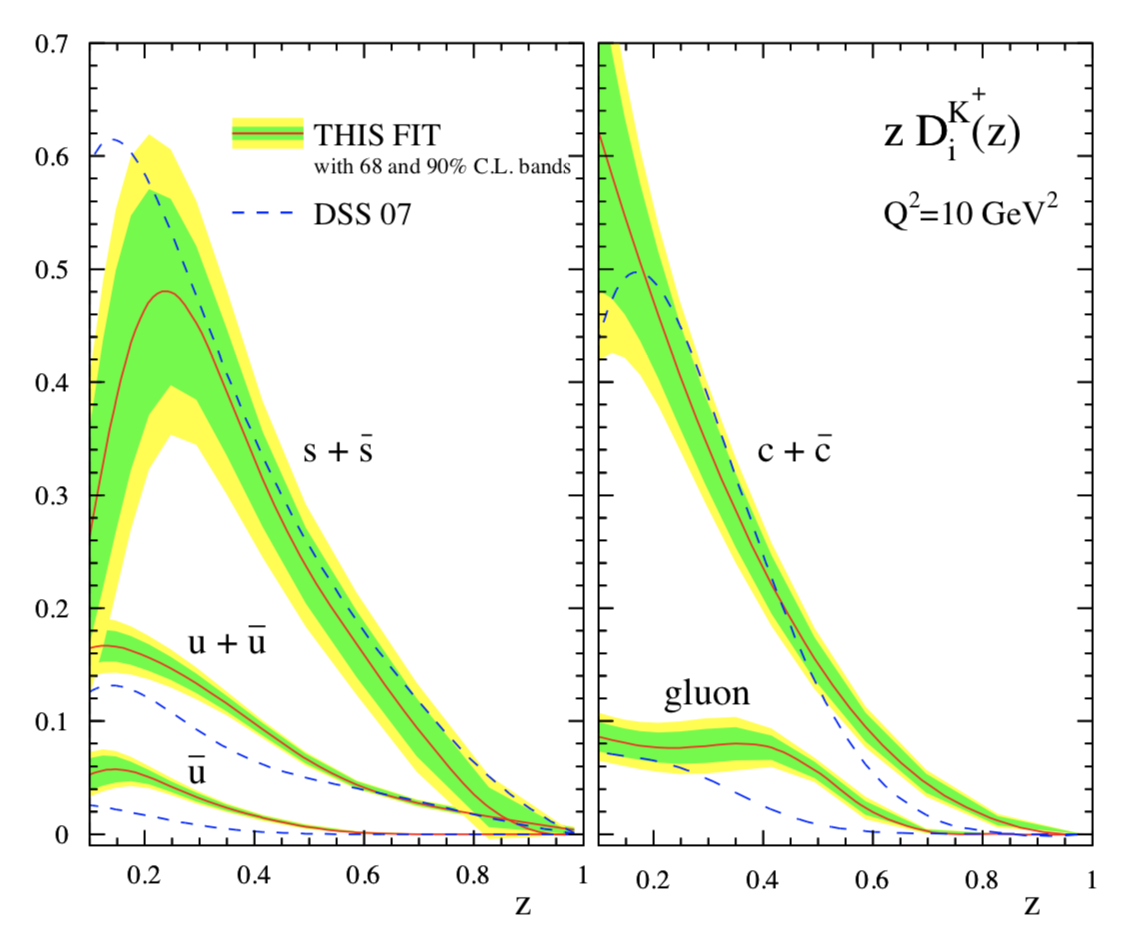
\includegraphics[scale=0.5]{./gfx/DSEHSK.png}
	\caption{Individual FFs for positively charged kaons $zD^{K^+}(z,Q^2)$ at $Q^2$ = 10 GeV$^2$ (solid lines) along with uncertainty estimates at 68\% and 90\% C.L. indicated by the inner and outer shaded bands, respectively. Also shown is a comparison to previous DSS07 global analysis\cite{DSS07} (dashed lines).}
	\label{pic:DSEHSK}
\end{figure}

\subsubsection*{JAM parametrization}

JAM is a Monte-Carlo based combined fit of PDFs and FFs using Bayesian statistics. In order to address some of the questions raised by the recent ambiguities in the strange quark FFs and their impact on the $\Delta s$ determination, they go beyond the standard fitting paradigm by performing the first Monte Carlo (MC) analysis of PDFs and FFs, extending the methodology of the iterative Monte-Carlo (IMC) approach already used for the analysis of spin-dependent PDFs\cite{IMC} to the case of FFs (Fig. \ref{pic:IMC}). The IMC approach allows for a full exploration of the parameter space when sampling initial priors for any chosen parametric form for the fitting function. It in consequence eliminates any bias introduced by fine-tuning or fixing specific parameters that are not well constrained by the data.


\begin{figure}[!h]
  \centering
	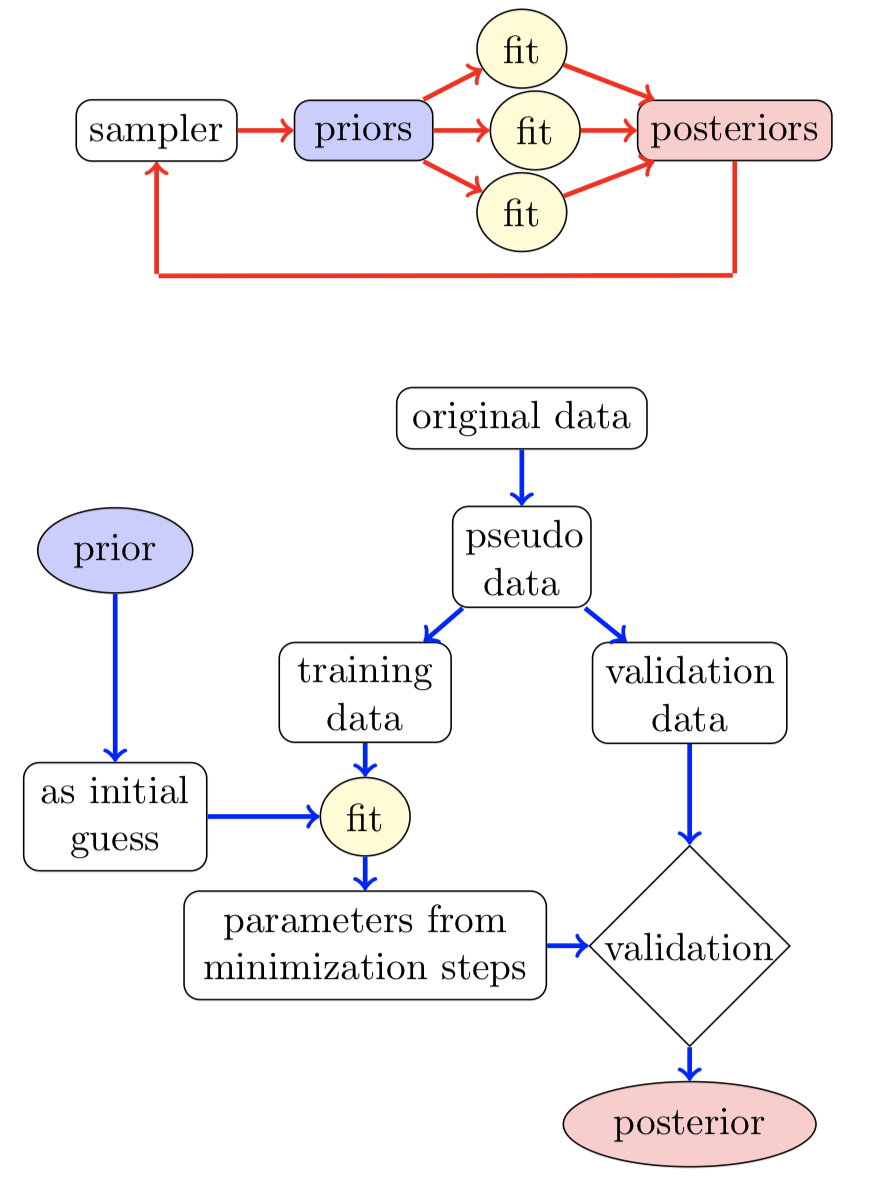
\includegraphics[scale=0.45]{./gfx/IMC.png}
	\caption{Workflow of the iterative Monte Carlo fitting strategy. In the upper diagram (red lines) an iteration begins at the prior sampler and a given number of fits are performed generating an ensemble of posteriors. After the initial iteration, with a flat sampler, the generated posteriors are used to construct a multivariate Gaussian sampler for the next iteration. The lower diagram (with blue lines) summarizes the workflow that transforms a given prior into a final posterior.}
	\label{pic:IMC}
\end{figure}


The functional they use for $D^h_q$ is the following :

\begin{equation}
  D^h_i (z,Q_0;\textbf{a}) = M \frac{z^{\alpha}(1-z)^{\beta}}{B(2+\alpha,1+\beta)}
  \label{eq:JAMparam}
\end{equation}

where $\textbf{a} = {M,\alpha,\beta,\gamma}$ is the vector of shape parameters to be fitted. The denominator is chosen so that the coefficient $M$ corresponds to the average momentum fraction $z$. Isospin symmetry is considered for all partons. Defining $D^{h^{+}}_{q^{\pm}}(z,Q^2) = D^{h^{+}}_{q}(z,Q^2) \pm D^{h^{+}}_{\bar{q}}(z,Q^2)$ allows JAM to consider only two template functions for the FFs $D^{\pi^{+}}_{u^{+}} = D^{\pi^{+}}_{d^{+}}$, $D^{K^{+}}_{u^{+}}$ and $D^{K^{+}}_{s^{+}}$ which contain both favoured and unfavoured distributions and only one template function for the rest of unfavoured distributions viz. $D^{\pi^{+}}_{\bar{u}} = D^{\pi^{+}}_{d}$, $D^{\pi^{+}}_{s} = (1/2)D^{\pi^{+}}_{s^{+}}$, $D^{K^{+}}_{\bar{u}} = (1/2)D^{K^{+}}_{d^{+}}$ and $D^{K^{+}}_{s}$ along with the heavy quarks and gluons.

The favoured and unfavoured FFs from DSS at LO for $Q^2$ = 5 GeV$^2$ are plotted as a function of $z$ for $\pi^+$ and $K^+$ (Fig. \ref{pic:JAMcomp}). The strange quark fragmentation into $K^+$ from JAM17 is compared with DSS07 and HKNS results. While part of the disagreement between fits can be explained by the different parametrizations used, the lack of data for kaon fragmentation function fits is an important factor explaining the discrepancy.

\begin{figure}[!h]
  \centering
	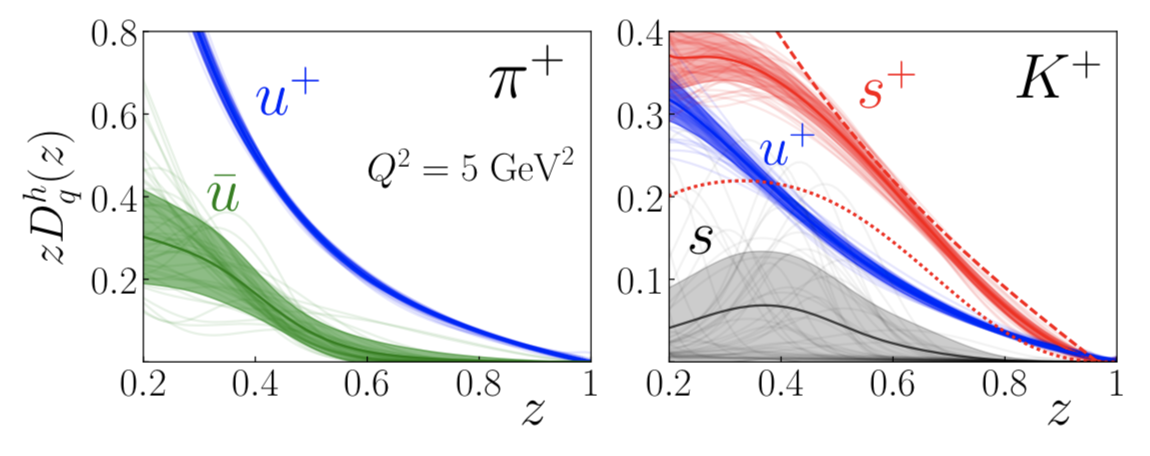
\includegraphics[scale=0.5]{./gfx/JAMcomp.png}
	\caption{Fragmentation functions $zD^h_q$ to $\pi^+$ (left panel) and $K^+$ (right panel) for $u^+$ (blue), $\bar{u}$ (green), $s^+$ (red) and $s$ (grey) at $Q^2$ = 5 GeV$^2$ for the JAM17 analysis, compared to $s^+ \rightarrow K^+$ from DSS07 and HKNS}
	\label{pic:JAMcomp}
\end{figure}

\newpage

\section{Summary}

The DIS process is a very interesting channel regarding the study of the nucleon structure. The unpolarized PDFs are well constrained in a wide kinematic domain for the first generation of quarks. Nevertheless going to higher masses, large uncertainties still subsist eg. for $s$ and $\bar{s}$. The FFs are a universal quantity which parametrize the quark hadronization. They can be measured via several processes and in particular SIDIS.

Multiple groups have already issued parametrization of quark FFs based on LO and NLO analyses of various data sets. They differ significantly in the strange quark sector. The COMPASS data presented in this thesis will provide a significant amount of new data which will help solving the discrepancies.
